%
% diffusion.tex
%
% (c) 2021 Prof Dr Andreas Müller, OST Ostschweizer Fachhochschule
%
\bgroup
\definecolor{darkgreen}{rgb}{0,0.6,0}
\begin{frame}[t]
\frametitle{Diffusion}
\vspace{-20pt}
\begin{columns}[t,onlytextwidth]
\begin{column}{0.48\textwidth}
\begin{center}
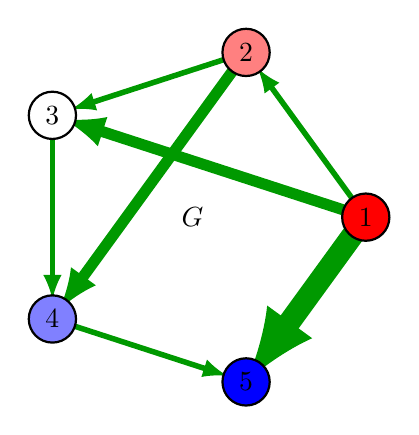
\begin{tikzpicture}[>=latex,thick]

\def\r{2.2}

\coordinate (A) at ({\r*cos(0*72)},{\r*sin(0*72)});
\coordinate (B) at ({\r*cos(1*72)},{\r*sin(1*72)});
\coordinate (C) at ({\r*cos(2*72)},{\r*sin(2*72)});
\coordinate (D) at ({\r*cos(3*72)},{\r*sin(3*72)});
\coordinate (E) at ({\r*cos(4*72)},{\r*sin(4*72)});

\draw[shorten >= 0.3cm,shorten <= 0.3cm] (A) -- (C);
\draw[color=white,line width=5pt] (B) -- (D);
\draw[shorten >= 0.3cm,shorten <= 0.3cm] (B) -- (D);

\draw[shorten >= 0.3cm,shorten <= 0.3cm] (A) -- (B);
\draw[shorten >= 0.3cm,shorten <= 0.3cm] (B) -- (C);
\draw[shorten >= 0.3cm,shorten <= 0.3cm] (C) -- (D);
\draw[shorten >= 0.3cm,shorten <= 0.3cm] (D) -- (E);
\draw[shorten >= 0.3cm,shorten <= 0.3cm] (E) -- (A);

\draw[->,color=darkgreen,line width=8pt,shorten <= 0.25cm,shorten >= 0cm]
	(A) -- (E);
\draw[->,color=darkgreen,line width=2pt,shorten <= 0.25cm,shorten >= 0.25cm]
	(A) -- (B);
\draw[->,color=darkgreen,line width=4pt,shorten <= 0.25cm,shorten >= 0.15cm]
	(A) -- (C);
\draw[->,color=darkgreen,line width=2pt,shorten <= 0.25cm,shorten >= 0.25cm]
	(B) -- (C);
\draw[->,color=darkgreen,line width=2pt,shorten <= 0.25cm,shorten >= 0.25cm]
	(C) -- (D);
\draw[->,color=darkgreen,line width=2pt,shorten <= 0.25cm,shorten >= 0.25cm]
	(D) -- (E);
\draw[->,color=darkgreen,line width=4pt,shorten <= 0.25cm,shorten >= 0.15cm]
	(B) -- (D);

\fill[color=red] (A) circle[radius=0.3];
\fill[color=red!50] (B) circle[radius=0.3];
\fill[color=white] (C) circle[radius=0.3];
\fill[color=blue!50] (D) circle[radius=0.3];
\fill[color=blue] (E) circle[radius=0.3];

\draw (A) circle[radius=0.3];
\draw (B) circle[radius=0.3];
\draw (C) circle[radius=0.3];
\draw (D) circle[radius=0.3];
\draw (E) circle[radius=0.3];

\node at (A) {$1$};
\node at (B) {$2$};
\node at (C) {$3$};
\node at (D) {$4$};
\node at (E) {$5$};
\node at (0,0) {$G$};

\end{tikzpicture}
\end{center}
\vspace{-10pt}
\begin{block}{Knotenfunktion}
$f\colon V\to \mathbb{R}$
\end{block}
\end{column}
\begin{column}{0.48\textwidth}
\begin{block}{Fluss}
Je grösser die Differenz zu den Nachbarn, desto grösser der Fluss in 
den Knoten:
\begin{align*}
\frac{df(v)}{dt}
&=
\kappa \sum_{\text{$v'$ Nachbar von $v$}} (f(v')-f(v))
\end{align*}
``Wärmeleitungsgleichung''
\end{block}
\end{column}
\end{columns}
\end{frame}
\egroup
